\documentclass{article}%
\usepackage[T1]{fontenc}%
\usepackage[utf8]{inputenc}%
\usepackage{lmodern}%
\usepackage{textcomp}%
\usepackage{lastpage}%
\usepackage{parskip}%
\usepackage[top=4cm,hmargin=2cm,headheight=65pt,footskip=65pt]{geometry}%
\usepackage{amsmath}%
\usepackage{graphicx}%
\usepackage{needspace}%
\usepackage{color}%
\usepackage{longtable}%
\usepackage{multirow}%
\usepackage[table]{xcolor}%
\usepackage{fancyhdr}%
\usepackage{tabularx}%
%
\definecolor{OsdagGreen}{HTML}{D5DF93}%
\fancypagestyle{header}{ 
\renewcommand{\headrulewidth}{0pt}%
\renewcommand{\footrulewidth}{0pt}%
\fancyhead{ 
}%
\fancyfoot{ 
}%
\fancyhead[C]{ 
\begin{tabularx}{\textwidth}{|l|p{6cm}|l|X|}%
\hline%
\rowcolor{OsdagGreen}%
Company Name&&Project Title&\\%
\hline%
\rowcolor{OsdagGreen}%
Group/Team Name&&Subtitle&\\%
\hline%
\rowcolor{OsdagGreen}%
Designer&&Job Number&\\%
\hline%
\rowcolor{OsdagGreen}%
Date&30 /05 /2020&Client&\\%
\hline%
\end{tabularx}
}%
\fancyfoot[R]{ 
Page \thepage\ of \pageref{LastPage}
}
}%
%
\begin{document}%
\normalsize%
\pagestyle{header}%
\section{Input Parameters}%
\label{sec:InputParameters}%
\renewcommand{\arraystretch}{1.2}%
\begin{longtable}{|p{5cm}|p{2cm}|p{2cm}|p{2cm}|p{5cm}|}%
\hline%
\hline%
\multicolumn{3}{|c|}{Module}&\multicolumn{2}{|c|}{Tension Members Bolted Design}\\%
\hline%
\hline%
\multicolumn{3}{|c|}{Axial (kN) *}&\multicolumn{2}{|c|}{200.0}\\%
\hline%
\hline%
\multicolumn{3}{|c|}{Length(mm) *}&\multicolumn{2}{|c|}{5000.0}\\%
\hline%
\hline%
\multicolumn{3}{|c|}{Section Size*}&\multicolumn{2}{|c|}{Ref List of Input Section}\\%
\hline%
\hline%
\multicolumn{5}{|c|}{\textbf{Bolt Details}}\\%
\hline%
\multicolumn{3}{|c|}{\multirow{3}{*}{Diameter (mm)*}}&\multicolumn{2}{|c|}{{[}8.0, 10.0, 12.0, 14.0, 16.0, 1}\\%
\multicolumn{3}{|c|}{\multirow{3}{*}{}}&\multicolumn{2}{|c|}{8.0, 20.0, 22.0, 24.0, 27.0, 3}\\%
\multicolumn{3}{|c|}{\multirow{3}{*}{}}&\multicolumn{2}{|c|}{0.0, 33.0, 36.0, 39.0{]}}\\%
\cline{4%
-%
5}%
\multicolumn{3}{|c|}{\multirow{2}{*}{Grade *}}&\multicolumn{2}{|c|}{{[}3.6, 4.6, 4.8, 5.6, 5.8, 6.8, }\\%
\multicolumn{3}{|c|}{\multirow{2}{*}{}}&\multicolumn{2}{|c|}{8.8, 9.8, 10.9, 12.9{]}}\\%
\cline{4%
-%
5}%
\hline%
\multicolumn{3}{|c|}{Type *}&\multicolumn{2}{|c|}{Bearing Bolt}\\%
\hline%
\hline%
\multicolumn{3}{|c|}{Bolt hole type}&\multicolumn{2}{|c|}{Standard}\\%
\hline%
\hline%
\multicolumn{3}{|c|}{Slip factor (µ\_f)}&\multicolumn{2}{|c|}{0.3}\\%
\hline%
\hline%
\multicolumn{3}{|c|}{Type of edges}&\multicolumn{2}{|c|}{a {-} Sheared or hand flame cut}\\%
\hline%
\hline%
\multicolumn{3}{|c|}{Gap between beam and <br>support (mm)}&\multicolumn{2}{|c|}{0.0}\\%
\hline%
\hline%
\multicolumn{3}{|c|}{Are the members exposed to <br>corrosive influences}&\multicolumn{2}{|c|}{False}\\%
\hline%
\hline%
\multicolumn{5}{|c|}{\textbf{Safety Factors {-} IS 800:2007 Table 5 (Clause 5.4.1) }}\\%
\hline%
\hline%
\multicolumn{3}{|c|}{Governed by Yielding}&\multicolumn{2}{|c|}{$\begin{aligned}\gamma_{m0}&=1.1\end{aligned}$}\\%
\hline%
\hline%
\multicolumn{3}{|c|}{Governed by Ultimate Stress}&\multicolumn{2}{|c|}{$\begin{aligned}\gamma_{m1}&=1.25\end{aligned}$}\\%
\hline%
\hline%
\multicolumn{3}{|c|}{Connection Bolts {-} Bearing Type}&\multicolumn{2}{|c|}{$\begin{aligned}\gamma_{mb}&=1.25\end{aligned}$}\\%
\hline%
\end{longtable}%
\subsection{List of Input Section}%
\label{subsec:ListofInputSection}%
\renewcommand{\arraystretch}{1.2}%
\begin{longtable}{|p{8cm}|p{8cm}|}%
\hline%
\multicolumn{1}{|c|}{Section Size*}&\multicolumn{1}{|c|}{{[}'MC 75', 'MC 100', 'MC 125', 'MC 125*', 'MC 150', 'MC 150*', 'MC 175', 'MC 175*', '}\\%
\hline%
\hline%
\multicolumn{1}{|c|}{ }&\multicolumn{1}{|c|}{MC 200', 'MC 200*', 'MC 225', 'MC 225*', 'MC 250', 'MC 250*', 'MC 250*', 'MC 300', }\\%
\hline%
\hline%
\multicolumn{1}{|c|}{ }&\multicolumn{1}{|c|}{'MC 300*', 'MC 300*', 'MC 350', 'MC 400', 'JC 100', 'JC 125', 'JC 150', 'JC 175', '}\\%
\hline%
\hline%
\multicolumn{1}{|c|}{ }&\multicolumn{1}{|c|}{JC 200', 'LC 75', 'LC 100', 'LC 125', 'LC (P) 125', 'LC 150', 'LC (P) 150', 'LC 175}\\%
\hline%
\hline%
\multicolumn{1}{|c|}{ }&\multicolumn{1}{|c|}{', 'LC 200', 'LC (P) 200', 'LC 225', 'LC 250', 'LC 300', 'LC (P) 300', 'LC 350', 'L}\\%
\hline%
\hline%
\multicolumn{1}{|c|}{ }&\multicolumn{1}{|c|}{C 400', 'MPC 75', 'MPC 100', 'MPC 125', 'MPC 125*', 'MPC 150', 'MPC 150*', 'MPC 175}\\%
\hline%
\hline%
\multicolumn{1}{|c|}{ }&\multicolumn{1}{|c|}{', 'MPC 175*', 'MPC 200', 'MPC 200*', 'MPC 225', 'MPC 225*', 'MPC 250', 'MPC 250*',}\\%
\hline%
\hline%
\multicolumn{1}{|c|}{ }&\multicolumn{1}{|c|}{ 'MPC 250*', 'MPC 300', 'MPC 300*', 'MPC 300*', 'MPC 350', 'MPC 400'{]}}\\%
\hline%
\end{longtable}

%
\Needspace{10\baselineskip}%
\newpage%
\section{Design Checks}%
\label{sec:DesignChecks}%
\subsection{Selected Member Data}%
\label{subsec:SelectedMemberData}%
\renewcommand{\arraystretch}{1.2}%
\begin{longtable}{|p{5cm}|p{2cm}|p{2cm}|p{2cm}|p{5cm}|}%
\hline%
\hline%
\multirow{14}{*}{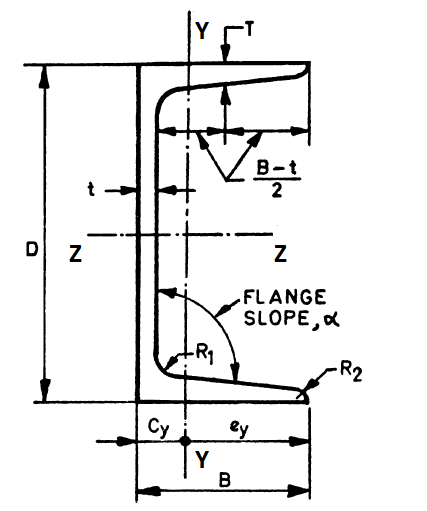
\includegraphics[width=5cm,height=5cm]{E:/workspace/Osdag3/ResourceFiles/images/Channel.png}}&\multicolumn{2}{|c|}{Section Size*}&\multicolumn{2}{|c|}{('JC 125', 'Channels')}\\%
\cline{2%
-%
5}%
&\multicolumn{2}{|c|}{Material *}&\multicolumn{2}{|c|}{E 250 (Fe 410 W)A}\\%
\cline{2%
-%
5}%
&\multicolumn{2}{|c|}{Ultimate strength, fu (MPa)}&\multicolumn{2}{|c|}{410}\\%
\cline{2%
-%
5}%
&\multicolumn{2}{|c|}{Yield Strength , fy (MPa)}&\multicolumn{2}{|c|}{250}\\%
\cline{2%
-%
5}%
&Mass&7.9&Iz(mm4)&2690000.0\\%
\cline{2%
-%
5}%
&Area(mm2) {-} A&1000.0&Iy(mm4)&251000.0\\%
\cline{2%
-%
5}%
&D(mm)&125&rz(mm)&51.7\\%
\cline{2%
-%
5}%
&B(mm)&50&ry(mm)&15.8\\%
\cline{2%
-%
5}%
&t(mm)&3.0&Zz(mm3)&43100.0\\%
\cline{2%
-%
5}%
&T(mm)&6.6&Zy(mm3)&7500.0\\%
\cline{2%
-%
5}%
&FlangeSlope&91.5&Zpz(mm3)&49100.0\\%
\cline{2%
-%
5}%
&R1(mm)&6.0&Zpy(mm3)&7500.0\\%
\cline{2%
-%
5}%
&R2(mm)&2.4&r(mm)&15.8\\%
\cline{2%
-%
5}%
&Cy(mm)&16.4&&\\%
\cline{2%
-%
5}%
\hline%
\end{longtable}

%
\newpage%
\subsection{Spacing Checks}%
\label{subsec:SpacingChecks}%
\renewcommand{\arraystretch}{1.2}%
\begin{longtable}{|p{2.5cm}|p{7.5cm}|p{3cm}|p{3cm}|}%
\hline%
\rowcolor{OsdagGreen}%
Check&Required&Provided&Remarks\\%
\hline%
\endhead%
\hline%
Min.Diameter (mm)&&$\begin{aligned} d &=14\end{aligned}$&\\%
\hline%
Hole Diameter (mm)& &$\begin{aligned} d_0 &=15\end{aligned}$&\\%
\hline%
Min. Gauge (mm)&$\begin{aligned}p/g_{min}&= 2.5 ~ d&\\ =&2.5*14.0&=35.0\end{aligned}$&35&Row Limit (rl) = 2\\%
\hline%
Min. Edge Distance (mm)&$\begin{aligned}e/e`_{min} &=[1.5~or~ 1.7] * d_0\\ &=1.7*15.0=25.5 \end{aligned}$&30&\\%
\hline%
Spacing Check&$\begin{aligned} depth & = 2 * e + (rl -1) * g \\ & = 2 * 30+(2-1)*35 \\ & = 95\end{aligned}$&99.8&Pass\\%
\hline%
\end{longtable}

%
\newpage%
\subsection{Member Checks}%
\label{subsec:MemberChecks}%
\renewcommand{\arraystretch}{1.2}%
\begin{longtable}{|p{2.5cm}|p{4.5cm}|p{8cm}|p{1cm}|}%
\hline%
\rowcolor{OsdagGreen}%
Check&Required&Provided&Remarks\\%
\hline%
\endhead%
\hline%
Tension Yielding Capacity (kN)&&$\begin{aligned}T_{dg}~or~A_c&= \frac{1 * A_g ~ f_y}{\gamma_{m0}}\\ &= \frac{1*1000.0*250}{1.1}\\ &= 227.27\end{aligned}$&\\%
\hline%
Tension Rupture Capacity (kN)&&$\begin{aligned}\beta &= 1.4 - 0.076*\frac{w}{t}*\frac{f_{y}}{0.9*f_{u}}*\frac{b_s}{L_c}\\ &\leq\frac{0.9*f_{u}*\gamma_{m0}}{f_{y}*\gamma_{m1}} \geq 0.7 \\ &= 1.4 - 0.076*\frac{50}{3.0}*\frac{250}{0.9*410}*\frac{92.0}{225 }\\ &\leq\frac{0.9* 410*1.1}{250*1.25} \geq 0.7 \\ &= 1.05\\ T_{dn} &= 1*(\frac{0.9*A_{nc}*f_{u}}{\gamma_{m1}} + \frac{\beta * A_{go} * f_{y}}{\gamma_{m0}})\\ &= 1*(\frac{0.9* 245.4*410}{1.25} + \frac{1.05*660.0*250}{1.1})\\ &= 229.94\end{aligned}$&\\%
\hline%
Block Shear Capacity (kN)&&$\begin{aligned}T_{db1} &= \frac{A_{vg} f_{y}}{\sqrt{3} \gamma_{m0}} + \frac{0.9 A_{tn} f_{u}}{\gamma_{m1}}\\ T_{db2} &= \frac{0.9*A_{vn} f_{u}}{\sqrt{3} \gamma_{m1}} + \frac{A_{tg} f_{y}}{\gamma_{m0}}\\ T_{db} &= min(T_{db1}, T_{db2})= 200.26\end{aligned}$&\\%
\hline%
Tension Capacity (kN)&200.0&$\begin{aligned} T_d &= min(T_{dg},T_{dn},T_{db})\\ &= min(227.27,229.94,200.26)\\ &=200.26\end{aligned}$&Pass\\%
\hline%
Slenderness&$\begin{aligned}\frac{K * L}{r} &\leq 400\end{aligned}$&$\begin{aligned}\frac{K * L}{r} &= \frac{1*5000.0}{15.8}\\ &= 316.46\end{aligned}$&Pass\\%
\hline%
Utilization Ratio&$\begin{aligned} Utilization~Ratio &\leq 1 \end{aligned}$&$\begin{aligned} Utilization~Ratio &= \frac{F}{Td}&=\frac{200.0}{200.26}\\ &= 1.0\end{aligned}$&\\%
\hline%
Axial Load Considered (kN)&$\begin{aligned} Ac_{min} &= 0.3 * A_c\\ &= 0.3 *227.27\\ &=68.18\\ Ac_{max} &=227.27\end{aligned}$&$\begin{aligned} A &=200.0\end{aligned}$&Pass\\%
\hline%
\end{longtable}

%
\newpage%
\subsection{Bolt Checks}%
\label{subsec:BoltChecks}%
\renewcommand{\arraystretch}{1.2}%
\begin{longtable}{|p{2.5cm}|p{5.5cm}|p{7cm}|p{1cm}|}%
\hline%
\rowcolor{OsdagGreen}%
Check&Required&Provided&Remarks\\%
\hline%
\endhead%
\hline%
Diameter (mm)&Bolt Quantity Optimisation&$\begin{aligned} d &=14\end{aligned}$&\\%
\hline%
Hole Diameter (mm)& &$\begin{aligned} d_0 &=15\end{aligned}$&\\%
\hline%
Grade&Bolt Grade Optimisation&3.6&\\%
\hline%
Bolt Ultimate Strength (N/mm2)&&$\begin{aligned} f_{ub} &=330.0\end{aligned}$&\\%
\hline%
Bolt Yield Strength (N/mm2)&&$\begin{aligned} f_{yb} &=190.0\end{aligned}$&\\%
\hline%
Nominal Stress Area (mm2)& &$\begin{aligned} A_{nb} &=115~( Ref~IS~1367-3~(2002))\end{aligned}$&\\%
\hline%
Kb& &$\begin{aligned} k_b & = min(\frac{e}{3*d_0},\frac{p}{3*d_0}-0.25,\frac{f_{ub}}{f_u},1.0)\\ & = min(\frac{30}{3*15.0},\frac{45}{3*15.0}-0.25,\frac{330.0}{410},1.0)\\ & = min(0.67,0.75,0.8,1.0)\\ & = 0.67\end{aligned}$&\\%
\hline%
Shear Capacity (kN)&&$\begin{aligned}V_{dsb} &= \frac{f_{ub} ~n_n~ A_{nb}}{\sqrt{3} ~\gamma_{mb}}\\ &= \frac{330.0*1*115}{\sqrt{3}~*~1.25}\\ &= 17.53\end{aligned}$&\\%
\hline%
Bearing Capacity (kN)&&$\begin{aligned}V_{dpb} &= \frac{2.5~ k_b~ d~ t~ f_u}{\gamma_{mb}}\\ &= \frac{2.5~*0.67*14.0*3.0*410}{1.25}\\ &=23.07\end{aligned}$&\\%
\hline%
Capacity (kN)&&$\begin{aligned}V_{db} &= min~ (V_{dsb}, V_{dpb})\\ &= min~ (17.53,23.07)\\ &=17.53\end{aligned}$&\\%
\hline%
No of Bolts&$\begin{aligned}R_{u} &= \sqrt{V_u^2+A_u^2}\\ n_{trial} &= R_u/ V_{bolt}\\ R_{u} &= \frac{\sqrt{0.0^2+200.0^2}}{17.53}\\ &=12\end{aligned}$&$\begin{aligned} n &=12\end{aligned}$&\\%
\hline%
No of Columns&&$\begin{aligned} n_c &=6\end{aligned}$&\\%
\hline%
No of Rows&&$\begin{aligned} n_r &=2\end{aligned}$&\\%
\hline%
Min. Pitch (mm)&$\begin{aligned}p/g_{min}&= 2.5 ~ d&\\ =&2.5*14.0&=35.0\end{aligned}$&45&Pass\\%
\hline%
Max. Pitch (mm)&$\begin{aligned}p/g_{max} &=\min(32~t,~300~mm)&\\ &=\min(32 *~3.0,~ 300 ~mm)\\&=96.0\\ where,&\\  t &= min(8.0,8.0)\end{aligned}$&45&Pass\\%
\hline%
Min. Gauge (mm)&$\begin{aligned}p/g_{min}&= 2.5 ~ d&\\ =&2.5*14.0&=35.0\end{aligned}$&35&Pass\\%
\hline%
Max. Gauge (mm)&$\begin{aligned}p/g_{max} &=\min(32~t,~300~mm)&\\ &=\min(32 *~3.0,~ 300 ~mm)\\&=96.0\\ where,&\\  t &= min(8.0,8.0)\end{aligned}$&35&Pass\\%
\hline%
Min. End Distance (mm)&$\begin{aligned}e/e`_{min} &=[1.5~or~ 1.7] * d_0\\ &=1.7*15.0=25.5 \end{aligned}$&30&Pass\\%
\hline%
Max. End Distance (mm)&$\begin{aligned}e/e`_{max} &= 12~ t~ \varepsilon&\\ \varepsilon &= \sqrt{\frac{250}{f_y}}\\ e/e`_{max}&=12 ~*3.0*\sqrt{\frac{250}{250}}\\ &=36.0\\ \end{aligned}$&30&Pass\\%
\hline%
Min. Edge Distance (mm)&$\begin{aligned}e/e`_{min} &=[1.5~or~ 1.7] * d_0\\ &=1.7*15.0=25.5 \end{aligned}$&32.4&Pass\\%
\hline%
Max. Edge Distance (mm)&$\begin{aligned}e/e`_{max} &= 12~ t~ \varepsilon&\\ \varepsilon &= \sqrt{\frac{250}{f_y}}\\ e/e`_{max}&=12 ~*3.0*\sqrt{\frac{250}{250}}\\ &=36.0\\ \end{aligned}$&32.4&Pass\\%
\hline%
Bolt Capacity post Long Joint (kN)&$\begin{aligned} &if~l\geq 15 * d~then~V_{rd} = \beta_{ij} * V_{db} \\ & if~l < 15 * d~then~V_{rd} = V_{db} \\ & where,\\ & l = ((nc~or~nr) - 1) * (p~or~g) \\ & \beta_{ij} = 1.075 - l/(200 * d) \\ & but~0.75\leq\beta_{ij}\leq1.0 \end{aligned}$&$\begin{aligned} l&= ((nc~or~nr) - 1) * (p~or~g) \\  &= (6 - 1) * 45=225\\  &= (2 - 1) * 35=35\\  l&= 225\\ & 15 * d = 15 * 14.0 = 210.0 \\ & since,~l \geq 15 * d~then~V_{rd} = \beta_{ij} * V_{db} \\ & \beta_{ij} = 1.075 - 225/(200*14.0) =0.99\\ & V_{rd} = 0.99 * 17.53=17.35 \end{aligned}$&\\%
\hline%
Capacity (kN)&16.67&17.35&Pass\\%
\hline%
\end{longtable}

%
\newpage%
\subsection{Gusset Plate Checks}%
\label{subsec:GussetPlateChecks}%
\renewcommand{\arraystretch}{1.2}%
\begin{longtable}{|p{2.5cm}|p{5cm}|p{7.5cm}|p{1cm}|}%
\hline%
\rowcolor{OsdagGreen}%
Check&Required&Provided&Remarks\\%
\hline%
\endhead%
\hline%
Min.Height (mm)&&$\begin{aligned} H &= 1* Depth + clearance \\ &=(1*125)+30.0\\ &= 155\end{aligned}$&\\%
\hline%
Min.Length (mm)&5000.0&$\begin{aligned} L &= (nc -1) * p + 2 * e\\ &= (6-1) *45+ (2 *30)\\ &= 285\end{aligned}$&Pass\\%
\hline%
Thickness (mm)&&$\begin{aligned} t_p &=8.0\end{aligned}$&\\%
\hline%
Tension Yielding Capacity (kN)&&$\begin{aligned} T_{dg} &= \frac{l*t*f_y}{\gamma_{mo}}\\ &=\frac{1*125*8.0*250}{1.1}\\ &=227.27\end{aligned}$&\\%
\hline%
Tension Rupture Capacity (kN)&&$\begin{aligned} T_{dn} &= \frac{0.9*A_{n}*f_u}{\gamma_{m1}}\\ &=\frac{0.9*(125-2*15.0)*8.0*410}{1.25}\\ &=224.35\end{aligned}$&\\%
\hline%
Block Shear Capacity (kN)&&$\begin{aligned}T_{db1} &= \frac{A_{vg} f_{y}}{\sqrt{3} \gamma_{m0}} + \frac{0.9 A_{tn} f_{u}}{\gamma_{m1}}\\ T_{db2} &= \frac{0.9*A_{vn} f_{u}}{\sqrt{3} \gamma_{m1}} + \frac{A_{tg} f_{y}}{\gamma_{m0}}\\ T_{db} &= min(T_{db1}, T_{db2})= 380.65\end{aligned}$&\\%
\hline%
Tension Capacity (kN)&$\begin{aligned} A &=200.0\end{aligned}$&$\begin{aligned} T_d &= min(T_{dg},T_{dn},T_{db})\\ &= min(227.27,224.35,380.65)\\ &=224.35\end{aligned}$&Pass\\%
\hline%
\end{longtable}

%
\Needspace{10\baselineskip}%
\newpage%
\section{3D View}%
\label{sec:3DView}%


\begin{figure}[h!]%
\centering%
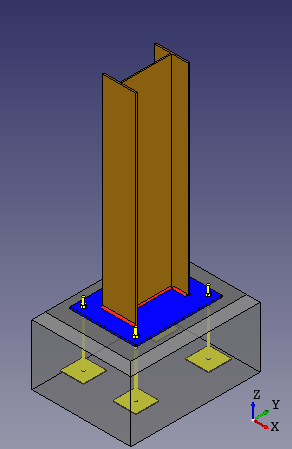
\includegraphics[width=\linewidth]{E:/workspace/Osdag3/ResourceFiles/images/3d.png}%
\caption{3D View}%
\end{figure}

%
\end{document}